% \documentclass[handout]{beamer}
\documentclass{beamer}
\usepackage[utf8]{inputenc}
\usepackage[T1]{fontenc}
\usepackage[square,numbers,authoryear]{natbib}
\usepackage{journals}
\usepackage{graphicx}
\usepackage{bibentry}

\usetheme{bart}

\graphicspath{%
{./figures/}%
}%

\beamertemplatetransparentcovered%

\title{Thesis presentation}
\subtitle{\textit{A new level of modelling of environmental effects on galaxies}}
\author{Manuel DUARTE}
\institute{Institut d'Astrophysique de Paris (IAP)\\Supervisor: Gary MAMON (IAP)}

\bartchapterimage{heic0206b_small.jpg}
\bartthumb{thumbs/heic0206b.png}
\begin{document}

%##################################################
% title page
%##################################################
\begin{frame}
    \titlepage%
\end{frame}

%##################################################
% Table of contents
%##################################################
\begin{frame}
    \tableofcontents%
\end{frame}

%##################################################
% Introduction
%##################################################
\section{Introduction}

\begin{frame}
    \frametitle{Introduction}
    % goal of the thesis
    \begin{block}{Thesis goal}
        Detailed understanding of the role of the environment on the properties
        of galaxies.
    \end{block}

    % how it is articulated
    \begin{block}{Organization}
        Two parts:
        \begin{enumerate}
            \item<1-> Quantify environments
            \item<2-> Physical intra-group processes
        \end{enumerate}
    \end{block}
\end{frame}

%##################################################
% Grouping algorithms
%##################################################
\section{Grouping algorithms}
\subsection{Who?}
\bartchapterimage{heic9910b_small.jpg}
\bartthumb{thumbs/heic9910b.png}
\begin{frame}

    \frametitle{Grouping algorithms}
    \framesubtitle{Who?}

    \begin{columns}
        \begin{column}{0.5\textwidth}
            \begin{block}{}
                \begin{enumerate}
                    \item<1-> Galaxies reside in different environments.
                    \item<2-> Previous studies: environment has little effect on galaxies.
                    \item<3-> Consequence of a bad quantification?
                \end{enumerate}
            \end{block}
        \end{column}
        \begin{column}{0.5\textwidth}
            % \includegraphics[height=0.8\textwidth]{amas.jpg}
        \end{column}
    \end{columns}

\end{frame}

%##################################################
% Mock catalogs
%##################################################
\section{Generating mock catalogues}
\bartchapterimage{heic0910i_small.jpg}
\bartthumb{thumbs/heic0910i.png}
\begin{frame}
    \frametitle{Generating mock catalogs}

    \begin{columns}
        \begin{column}{0.5\textwidth}
            % 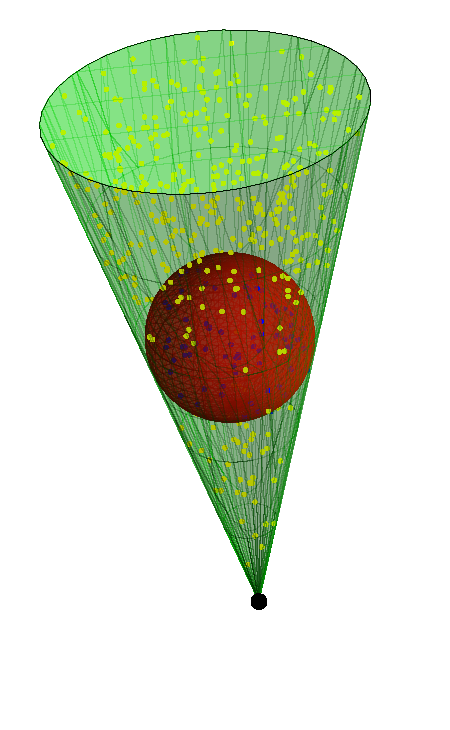
\includegraphics[height=0.8\textheight,angle=-90]{cone.pdf}
        \end{column}
        \begin{column}{0.5\textwidth}
            \begin{alertblock}{Mock catalogs}
                \begin{enumerate}
                    \item<1-> Allow to link redshift space selected groups
                        to real space groups.
                    \item<2-> Constructed from galaxy catalog output of
                        semi-analytical codes applied on Millennium-II run
                        and HOD (halo occupation distribution).
                    \item<3-> Similar to SDSS survey: mask, observational
                        uncertainties\ldots
                \end{enumerate}
            \end{alertblock}
        \end{column}
    \end{columns}
\end{frame}

%##################################################
% FoF
%##################################################
\section{Friends-of-Friends algorithm}
\bartchapterimage{heic1006a_small.jpg}
\bartthumb{thumbs/heic1006a.png}
\begin{frame}

    \frametitle{Friends-of-Friends algorithm}

    \begin{columns}
        \begin{column}{0.65\textwidth}
        \end{column}
        \begin{column}{0.35\textwidth}
            \only<1>{%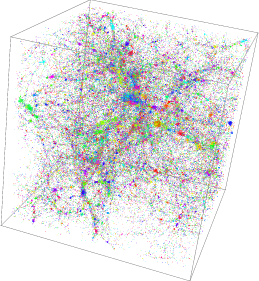
\includegraphics[width=\textwidth]{cubemock.png}}
            }
            \only<2>{%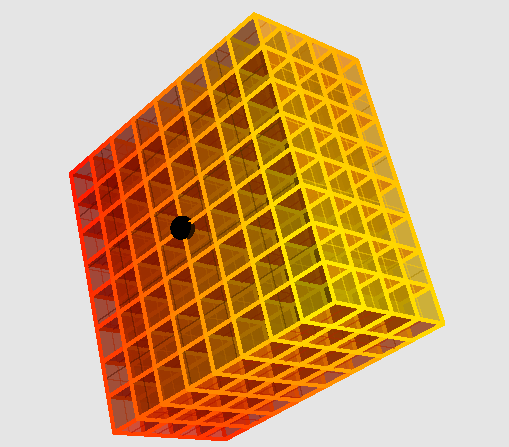
\includegraphics[width=\textwidth]{mock.pdf}}
            }
        \end{column}
    \end{columns}
\end{frame}

%##################################################
% MAGGIE
%##################################################
\section{MAGGIE}
\bartchapterimage{heic1302a_small.jpg}
\bartthumb{thumbs/heic1302a.png}
\begin{frame}
    \frametitle{MAGGIE}
    \begin{columns}
        \begin{column}{0.45\textwidth}
            % \includegraphics[width=\textwidth]{projSDSS.pdf}
        \end{column}
        \begin{column}{0.55\textwidth}
            \begin{block}{Compare with other galaxy group algorithms}
                \begin{enumerate}
                    \item \citet{Yang+07}.
                    \item \citet{Berlind+06}.
                    \item \citet{DominguezRomero+12}.
                \end{enumerate}
            \end{block}
        \end{column}
    \end{columns}
    \begin{block}{Applications}
        \begin{itemize}
            \item Apply algorithm on SDSS survey.
            \item Observe environment effects on galaxies.
        \end{itemize}
    \end{block}
\end{frame}

\bibliographystyle{unsrtnat}
\nobibliography{references}

\end{document}
